\begin{frame}[fragile]{Factory}
To choose the \verb|Algorithm| at runtime:
\begin{verbatim}
template<class AbstractProduct, typename... Args>
class Factory{
private:
    std::map<Identifier, Builder> storage;
    //[...]
public:
    static Factory& Instance();
    std::unique_ptr<AbstractProduct> create_object(
        const Identifier &name, Args... args) const;
    void add_builder(const Identifier &name,
        const Builder &builder);
    //[...]
}
\end{verbatim}
\end{frame}


\begin{frame}[fragile] {Protocol Buffers API}
\begin{itemize}
	\item For multivariate data storage
	\item Model in \texttt{output.proto}:
\end{itemize}
\begin{small}
\begin{verbatim}
        message Par_Col {
            repeated double elems = 1;
        }
        message Param {
            repeated Par_Col par_cols = 1;
        }
        message UniqueValues {
            repeated Param params = 1;
        }
        message IterationOutput {
            repeated int32 allocations = 1;
            repeated UniqueValues uniquevalues = 2;
        }
        message ChainOutput {
            repeated IterationOutput chain = 1;
        }
\end{verbatim}
\end{small}
\end{frame}


\begin{frame}{Collectors}
	\begin{center}
		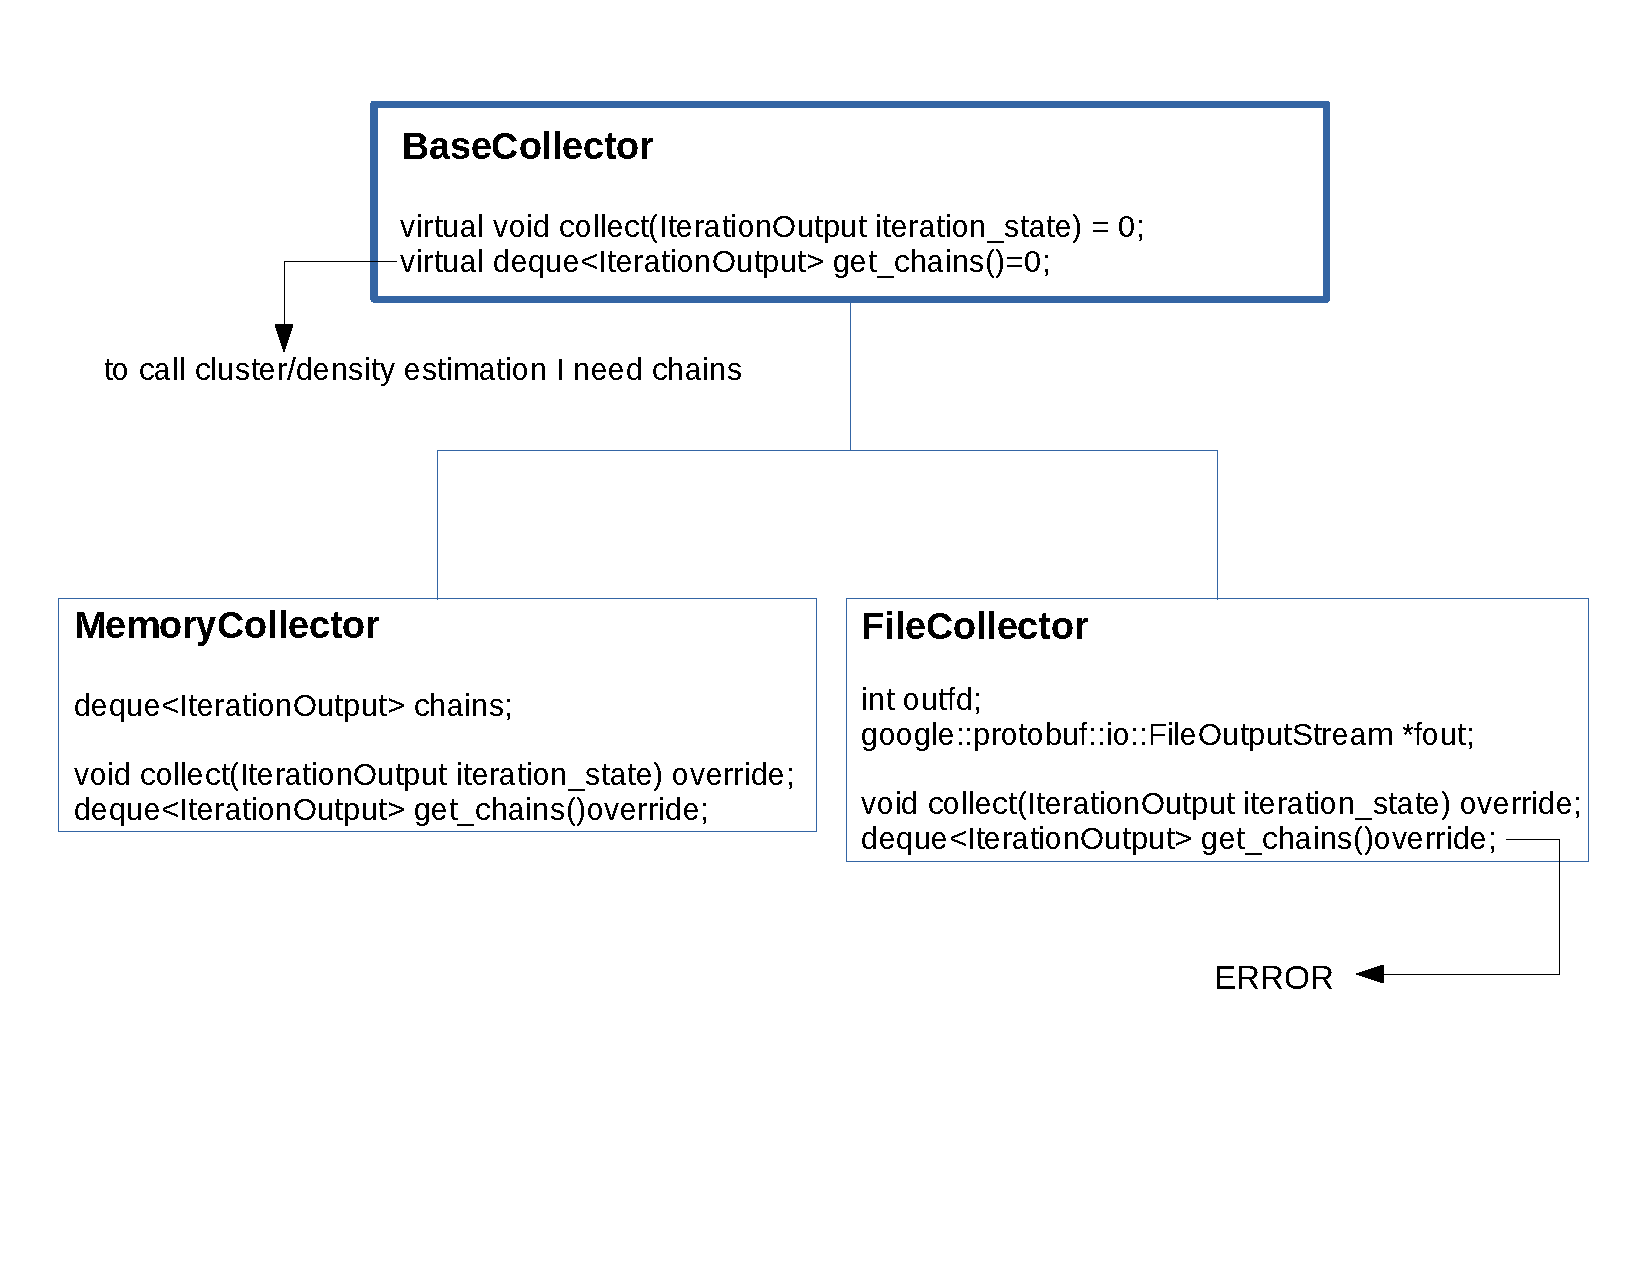
\includegraphics[scale=0.35]{etc/collectors.pdf}
	\end{center}
\end{frame}
